\chapter{การพยากรณ์ (Forecasting)}

การพยากรณ์ (Forecasting) คือการใช้ข้อมูลของสิ่งที่สนใจที่เกิดขึ้นในอดีตเพื่อสร้างแบบจำลองคณิตศาสตร์ที่ใช้ในการคำนวณสิ่งที่สนใจนั้นในอนาคต และในบางตำราจะยังรวมถึงการใช้สภาวะการณ์ที่สำรวจได้ในปัจจุบันรวมไปถึงในอดีตเพื่อทำนาย (Prediction) ค่าที่สนใจ ตัวอย่างเช่น
\begin{itemize}
    \item ฝ่ายขายใช้ยอดขายย้อนหลัง 12 เดือนเพื่อทำนายยอดขายในเดือนถัดไป
    \item ทีมการตลาดต้องการทำนายความต้องการซื้อสินค้าบางอย่างของลูกค้าโดยอาศัยคุณลักษณะต่าง ๆ เช่นเพศ อายุ ฐานเงินเดือน สินค้าที่ซื้อในเดือนที่แล้ว เป็นต้น
\end{itemize}

ในรายวิชานี้ เราจะศึกษา 2 รูปแบบการทำนายหลัก ๆ ดังนี้
\begin{figure}[h]
    \centering
    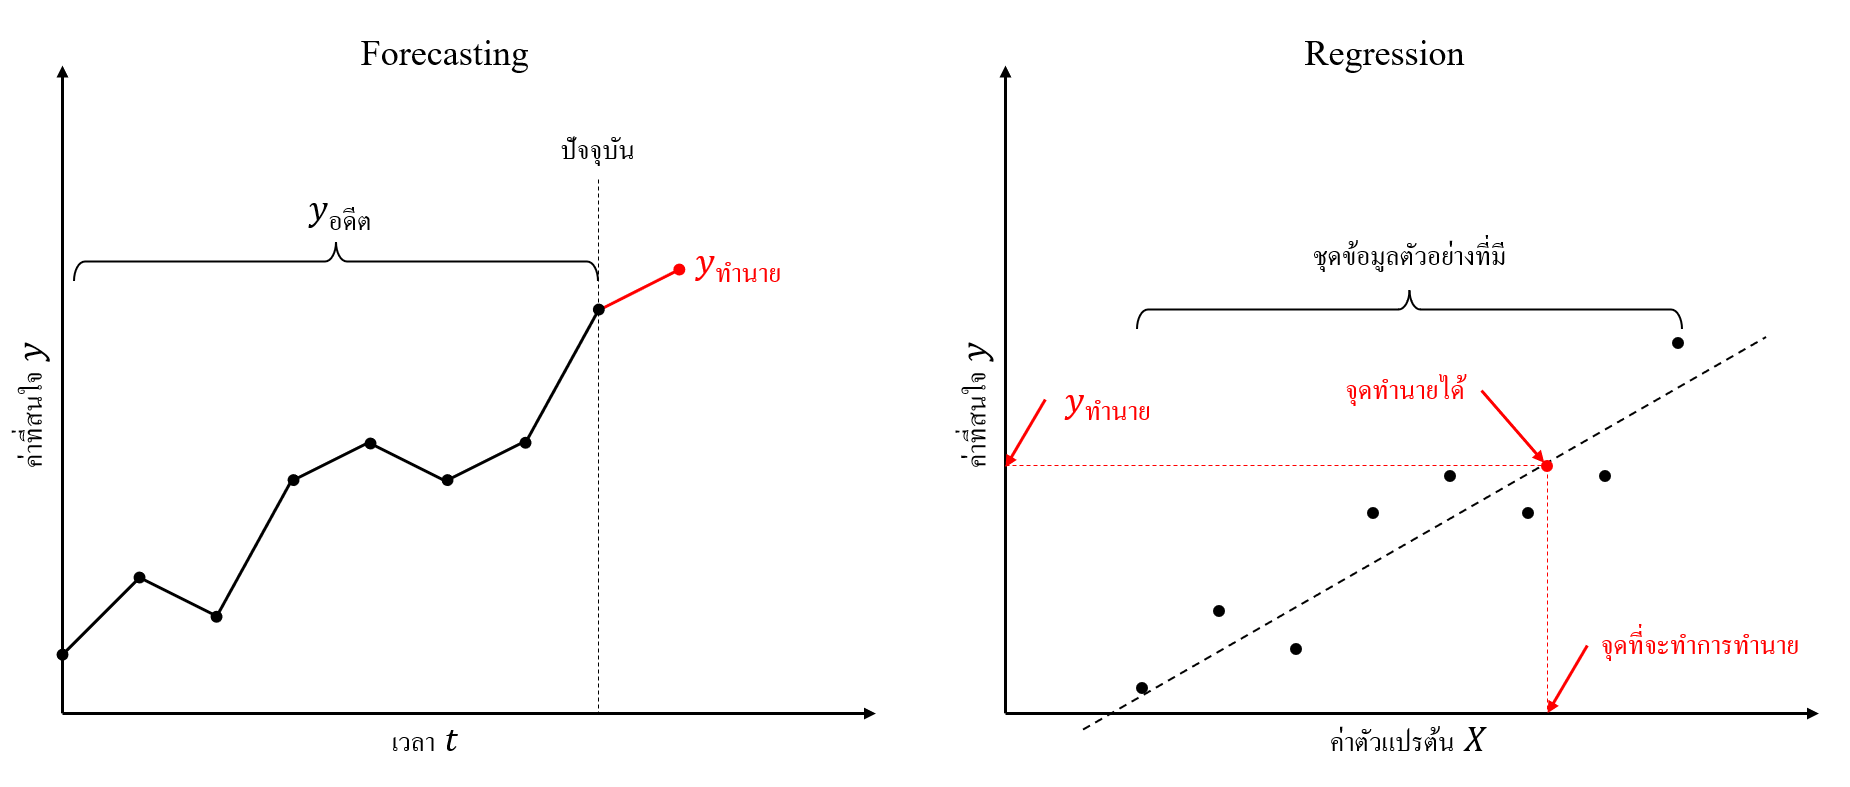
\includegraphics[width=1\linewidth]{forecast_and_regression.png}
    \caption{ความแตกต่างระหว่างตัวแบบอนุกรมเวลาและตัวแบบถดถอย}
\end{figure}
\begin{enumerate}
    \item \textbf{ตัวแบบอนุกรมเวลา} (time series forecasting): เป็นตัวแบบที่อยู่บนสมมติฐานว่าตัวแปรที่เราสนใจมีค่าขึ้นอยู่กับตัวแปรเดียวกันที่เกิดขึ้นในอดีต
    \[
        \hat{y}_{t} \sim y_{t-1}, y_{t-2}, \dots, y_{t-k} 
    \]
    \item \textbf{ตัวแบบการถอดถอย} (regression model): เป็นตัวแบบที่อยู่บนสมมติฐานว่าตัวแปรที่เราสนใจมีค่าขึ้นอยู่กับตัวแปรอื่น ๆ ที่เกิดขึ้นพร้อมกัน (หรือเป็นอยู่)
    \[
        \hat{y}_{t} \sim x_{1,t}, x_{2,t}, \dots, x_{n,t} 
    \]
\end{enumerate}

ทั้งนี้ เราไม่สามารถบอกได้ว่าวิธีการใดเป็นวิธีการที่ดีที่สุด เพราะแต่ละวิธีการ (ที่กำลังจะกล่าวในหัวข้อถัดไป) มีสมมติฐานตั้งต้นที่แตกต่างกัน ขึ้นอยู่กับลักษณะของข้อมูลว่าจะเหมาะสมกับตัวแบบไหน แต่ในทางปฏิบัติ ถ้าไม่มีได้ติดขัดเรื่องปัญหาด้านทรัพยากรในการทำการคำนวณ เรามักจะลองทุกวิธีการและวัดผลเพื่อตรวจสอบเปรียบเทียบความสามารถของแต่ละตัวแบบ (เรียนในหัวข้อสุดท้าย)

%\subsection{ข้อตกลงเรื่องสัญลักษณ์}

\section{ตัวแบบอนุกรมเวลา}
\subsection{วิธีการค่าเฉลี่ยรวม}
\begin{itemize}
    \item เหมาะกับข้อมูลที่มีลักษณะที่ค่อนข้างคงที่ในภาพรวม (ไม่ได้มีแนวโน้มที่เปลี่ยนแปลงไปเช่นตลาดโตขึ้นเรื่อย ๆ)
    \item วิธีการคำนวณ:
    \[
    \hat{y}_{t+1} = \frac{\sum_{i=1}^{t} y_i}{t} = \frac{y_1 + y_2 + \cdots + y_t}{t}
    \]
\end{itemize}

\begin{example}
    {วิธีการค่าเฉลี่ยรวม}{}
    บริษัทหนึ่งมีความต้องการทำนายยอดขายในเดือนที่ 7 โดยที่มียอดขาย 6 เดือนที่ผ่านมาตามตารางด้านล่างนี้ ทั้งนี้ ลองหาค่าทำนายของแต่ละเดือนก่อนหน้าด้วย
\end{example}
\begin{tabular}{|c|c|}
\hline
เดือน & ยอดขาย \\ \hline
1     & 800    \\ \hline
2     & 900    \\ \hline
3     & 800    \\ \hline
4     & 1000   \\ \hline
5     & 1000   \\ \hline
6     & 1300   \\ \hline
\end{tabular}
\newpage
\subsection{วิธีค่าเฉลี่ยเคลื่อนที่ (Moving Average)}
\begin{itemize}
    \item ถ้าข้อมูลระยะยาวไม่คงที่ วิธีการหาค่าเฉลี่ยทั้งหมดอาจจะเอาผลที่ไกลเกินไปมารวม
    \item แต่ถ้าพบว่ามีความคงที่ในระยะสั้น ๆ เช่น ในช่วง 6 เดือนไม่ได้มีการเปลี่ยนแปลงมากนัก เราก็ควรนำแค่ 6 เดือนย้อนหลังมาคิด ซึ่งจะเรียกว่าการหาค่าเฉลี่ยเคลื่อนที่ย้อนหลัง 6 เดือน
    \item วิธีการคำนวณ:
    \[
    \hat{y}_{t+1} = \frac{\sum_{i=t-n+1}^{t} y_i}{n} = \frac{y_{t-n+1} + y_{t-n+2} + \cdots + y_t}{n}
    \]
\end{itemize}
\begin{example}
    {วิธีการค่าเฉลี่ยเคลื่อนที่}{}
    จากตารางเดิม จงหาค่าเฉลี่ยเคลื่อนที่ 3 เดือน และค่าเฉลี่นเคลื่อนที่ 4 เดือนของเดือนทั้งหมดที่เป็นไปได้จนถึงเดือนที่ 7
\end{example}
\begin{tabular}{|c|c|}
\hline
เดือน & ยอดขาย \\ \hline
1     & 800    \\ \hline
2     & 900    \\ \hline
3     & 800    \\ \hline
4     & 1000   \\ \hline
5     & 1000   \\ \hline
6     & 1300   \\ \hline
\end{tabular}\\
~
\vspace{1cm}\\
\noindent\begin{tabular}{|c|c|}
\hline
เดือน & ยอดขาย \\ \hline
1     & 800    \\ \hline
2     & 900    \\ \hline
3     & 800    \\ \hline
4     & 1000   \\ \hline
5     & 1000   \\ \hline
6     & 1300   \\ \hline
\end{tabular}
\newpage
\subsection{วิธีค่าเฉลี่ยเคลื่อนที่ถ่วงน้ำหนัก (Weighted Moving Average)}
\begin{itemize}
    \item เป็นวิธีการที่ต่อยอดมาจากการทำค่าเฉลี่ยนเคลื่อนที่ แต่มีแนวคิดว่าผลกระทบที่ยิ่งห่างออกไปยิ่งควรมีความสำคัญน้อยลง แต่ในขณะที่เหตุการณ์ล่าสุดควรมีผลกระทบมากที่สุด
    \item วิธีการถ่วงน้ำหนักที่ง่ายที่สุดคือไล่ 1, 2, 3, ... จากอดีตสุดมาปัจจุบันสุด
    \item เรียกอีกชื่อว่า \textbf{วิธีปรับเรียบแบบเชิงเส้น}
    \item วิธีการคำนวณ:
    \[
    \hat{y}_{t+1} = \frac{\sum_{i=t-n+1}^{t} (i-t+n)y_i}{\sum_{i=1}^n i} = \frac{1 \cdot y_{t-n+1} + 2 \cdot y_{t-n+2} + \cdots + n \cdot y_t}{1 + 2 + \cdots + n}
    \]
\end{itemize}
\begin{example}
    {วิธีการค่าเฉลี่ยเคลื่อนที่ถ่วงน้ำหนัก}{}
    จากตารางเดิม จงหาค่าเฉลี่ยเคลื่อนที่ถ่วงน้ำหนัก 3 เดือน และค่าเฉลี่นเคลื่อนที่ถ่วงน้ำหนัก 4 เดือนของเดือนทั้งหมดที่เป็นไปได้จนถึงเดือนที่ 7
\end{example}
\begin{tabular}{|c|c|}
\hline
เดือน & ยอดขาย \\ \hline
1     & 800    \\ \hline
2     & 900    \\ \hline
3     & 800    \\ \hline
4     & 1000   \\ \hline
5     & 1000   \\ \hline
6     & 1300   \\ \hline
\end{tabular}\\
~
\vspace{1cm}\\
\noindent\begin{tabular}{|c|c|}
\hline
เดือน & ยอดขาย \\ \hline
1     & 800    \\ \hline
2     & 900    \\ \hline
3     & 800    \\ \hline
4     & 1000   \\ \hline
5     & 1000   \\ \hline
6     & 1300   \\ \hline
\end{tabular}

\newpage
\subsection{วิธีปรับเรียบแบบเอกซ์โพเนเชียล (exponential smoothing)}
\begin{itemize}
    \item เป็นอีกวิธีในการถ่วงน้ำหนัก โดยให้ความสำคัญของค่าล่าสุดเริ่มที่ 1 และลดค่าความสำคัญลงไปแบบ exponential โดยที่ยังมีการนำค่าตั้งแต่จุดเริ่มต้นมาพิจารณา
    \item แต่สูตรการคำนวณถูกจัดให้อยู่ในรูปที่คำนวณได้ง่าย (แค่ต้องคำนวณไต่ลำดับขึ้นมาเรื่อย ๆ) รูปแบบ exponential จึงไม่เห็นอยู่ในสูตร
    \item วิธีการคำนวณ:
    \[
    \hat{y}_{t+1} = \hat{y}_{t} + \alpha(y_t - \hat{y}_{t})
    \]
    หรือ
    \[
    \hat{y}_{t+1} = \alpha y_{t} + (1-\alpha)\hat{y}_t
    \]
    โดยที่ $0 \leq \alpha \leq 1$
    \item ค่า $\alpha$ เป็นค่าที่ต้องกำหนดขึ้นมาตั้งแต่เริ่มตัดสินใจ (เหมือนกับที่เราต้องเลือกว่าจะ moving average หรือ weighted moving average ของกี่เดือน)
\end{itemize}
\begin{example}
    {วิธีปรับเรียบแบบเอกซ์โพเนนเชียล}{}
    จากตารางเดิม จงหาค่าทำนายจากวิธีการปรับเรียบแบบเอกซ์โพเนนเชียล โดยใช้ $\alpha=0.3$ และ $\alpha=0.8$
\end{example}
\begin{tabular}{|c|c|}
\hline
เดือน & ยอดขาย \\ \hline
1     & 800    \\ \hline
2     & 900    \\ \hline
3     & 800    \\ \hline
4     & 1000   \\ \hline
5     & 1000   \\ \hline
6     & 1300   \\ \hline
\end{tabular}\\
~
\vspace{1cm}\\
\noindent\begin{tabular}{|c|c|}
\hline
เดือน & ยอดขาย \\ \hline
1     & 800    \\ \hline
2     & 900    \\ \hline
3     & 800    \\ \hline
4     & 1000   \\ \hline
5     & 1000   \\ \hline
6     & 1300   \\ \hline
\end{tabular}

\newpage
\begin{remark}
    {สาเหตุที่เรียกว่าการปรับเรียบแบบเอกซ์โพเนนเชียล}{}
    รูปแบบสมการที่นิยามมาในด้านบนเรียกว่าการนิยามแบบเวียนเกิด คือการจะหาพจน์ที่ใด ๆ ได้ จะต้องคำนวณให้ทราบค่าพจน์ก่อนหน้าก่อน ดังนั้นจึงจำเป็นต้องคำนวณไล่จากขั้นที่ 1 ขึ้นมาจนถึงขั้นที่ต้องการ แต่ทั้งนี้ เรายังสามารถจัดรูปให้อยู่ในรูปที่ไม่ขึ้นกับพจน์ก่อนหน้าได้ดังนี้
    \begin{align*}
        \hat{y}_{t+1}   &= \alpha y_{t} + (1-\alpha)\hat{y}_t\\
                        &= \alpha y_{t} + (1-\alpha)(\alpha y_{t-1} + (1-\alpha)\hat{y}_{t-1})\\
                        &= \alpha y_{t} + \alpha (1-\alpha) y_{t-1} + (1-\alpha)^2 \hat{y}_{t-1}\\
                        &= \alpha y_{t} + \alpha (1-\alpha) y_{t-1} + \alpha (1-\alpha)^2 y_{t-2} + (1-\alpha)^3 \hat{y}_{t-3}\\
                        &= \alpha y_{t} + \alpha (1-\alpha) y_{t-1} + \alpha (1-\alpha)^2 y_{t-2} + \alpha (1-\alpha)^3 y_{t-3} + (1-\alpha)^4 \hat{y}_{t-4}\\
                        & \quad\vdots \\
                        &= \alpha y_{t} + \alpha (1-\alpha) y_{t-1} + \alpha (1-\alpha)^2 y_{t-2} + \cdots + \alpha (1-\alpha)^{t-2} y_2 + (1 - \alpha)^{t-1} y_1
    \end{align*}
    หรือถ้าเขียนเป็นตัวอย่างแบบตัวเลขชัดเจน จะมีดังนี้
    \begin{align*}
        \hat{y}_1 &= y_1\\
        \hat{y}_2 &= (1 - \alpha)^0 y_1 = y_1\\
        \hat{y}_3 &= \alpha y_2 + (1-\alpha) y_1\\
        \hat{y}_4 &= \alpha y_3 + \alpha (1-\alpha) y_2 + (1-\alpha)^2 y_1\\
        \hat{y}_5 &= \alpha y_4 + \alpha (1-\alpha) y_3 + \alpha (1-\alpha)^2 y_2 + (1-\alpha)^3 y_1
    \end{align*}
    ซึ่งจะเห็นว่า
    \begin{enumerate}
        \item จำนวนพจน์ของค่าจริงที่มาใช้คำนวณจะไม่ถูกกำหนดตายตัวเหมือนวิธีค่าเฉลี่ยเคลื่อนที่แบบอื่นๆ
        \item แต่ความสำคัญก็จะถูกลดทอนลงเรื่อย ๆ จนเข้าใกล้ 0
    \end{enumerate}
    ตัวอย่างกราฟค่าความสำคัญเมื่อใช้ $\alpha = 0.3, 0.5, 0.95, 1$ แสดงการลดแบบ exponential\\
    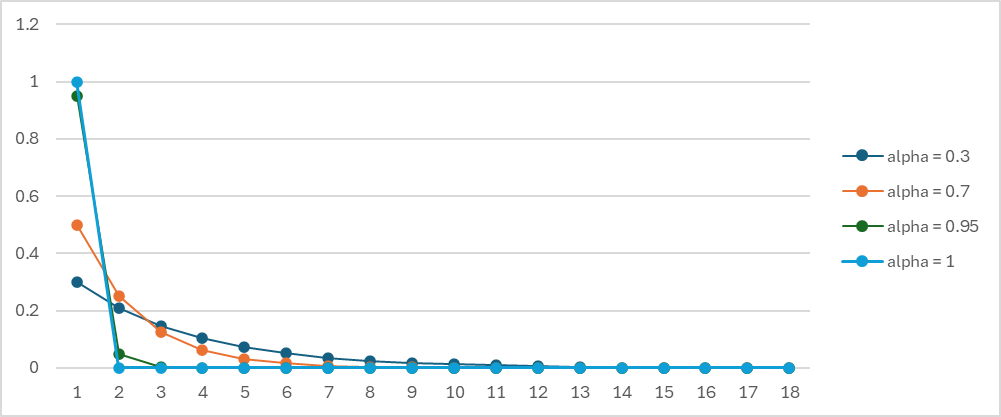
\includegraphics[width=0.9\linewidth]{alpha-expo-smoothing.png}
\end{remark}

\section{ตัวแบบการถดถอยเชิงเส้น}
\begin{itemize}
    \item ตัวแบบการถดถอย (regression) เป็นการสร้างตัวแบบการทำนายโดยอยู่บนสมมติฐานว่าตัวแปรต้นตัวหนึ่ง ($x$) มีความสัมพันธ์เชิงฟังก์ชันกับค่าตัวแปรที่เราสนใจ ($y$)
    \item ในวิชานี้เราสนใจแค่การถดถอยเชิงเส้นตัวแปรเดียว กล่าวคือ มีชุดข้อมูล $(x_1,y_1), (x_2, y_2), \dots, (x_n,y_n)$ ที่มีความสัมพันธ์
    $$
    Y = a_0 + a_1X + \epsilon
    $$
    โดย $a_0, a_1$ เป็นค่าคงที่ และ $\epsilon$ คือพจน์ค่าคาดเคลื่อน
    \item เป้าหมายคือเราต้องการประมาณค่า $a_0 = \alpha_0, a_1 = \alpha_1$ ที่
    $$
    Y \approx \hat{Y} = \alpha_0 + \alpha_1X
    $$
\end{itemize}
\begin{figure}[h]
    \centering
    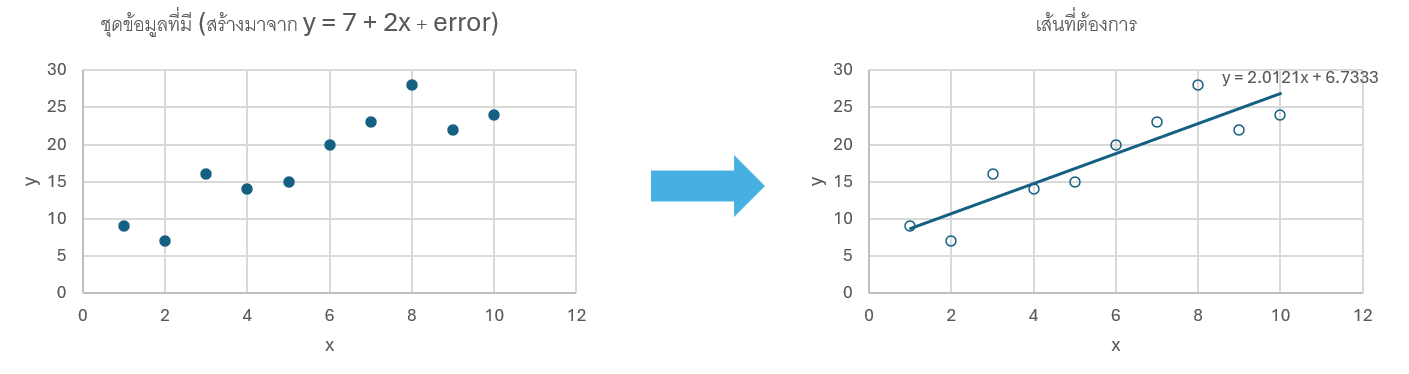
\includegraphics[width=1\linewidth]{regressionSample.png}
\end{figure}

\begin{algorithm}[breakable]
    {}{}
    ค่า $a_0, a_1$ ของตัวแบบการถดถอยเชิงเส้น $Y = a_0 + a_1X + \epsilon$ ของชุดข้อมูล $(x_1,y_1), (x_2, y_2), \dots, (x_n,y_n)$ สามารถประมาณค่าได้ด้วย $\alpha_0, \alpha_1$ (ด้วยวิธีการทางคณิตศาสตร์ที่เรียกว่าวิธีกำลังสองต่ำสุด (Least Squared Error)) ตามสูตร
	\[
        \alpha_1 = \frac{\sum_{i=1}^n(x_i-\bar{x})(y_i-\bar{y})}{\sum_{i=1}^n (x_i - \bar{x})^2},\hspace{1cm} \alpha_0 = \bar{y} - \alpha_1 \bar{x}
	\]
    และจะได้ว่า $\hat{Y} = \alpha_0 + \alpha_1X$ เป็นตัวแบบการถดถอยเชิงเส้นของ $Y = a_0 + a_1X + \epsilon$
    
    โดยขั้นตอนการคำนวณตามสูตรดังกล่าวคือ
   	\begin{enumerate}
   		\item คำนวณหาค่าเฉลี่ย $\bar{x} = \sum_{i=1}^{n}x / n$ และค่าเฉลี่ย $\bar{y} = \sum_{i=1}^{n}y / n$
   		\item $(x_i-\bar{x})$: คำนวณหาผลต่างระหว่างค่า $x$ และค่าเฉลี่ย $\bar{x}$ ของทุกข้อมูล 
   		\item $(y_i-\bar{y})$: คำนวณหาผลต่างระหว่างค่า $y$ และค่าเฉลี่ย $\bar{y}$ ของทุกข้อมูล 
   		\item $(x_i-\bar{x})(y_i-\bar{y})$: นำค่าผลต่างจาก 2 ข้อก่อนหน้ามาคูณกัน
   		\item $\sum_{i=1}^n(x_i-\bar{x})(y_i-\bar{y})$: นำค่าผลคูณของทุกข้อมูลจากขั้นที่ผ่านมามาบวกกัน
   		\item $(x_i-\bar{x})^2$: นำค่าผลต่างที่คำนวณไว้ในขั้นที่ 2 มายกกำลังสอง
   		\item $\sum_{i=1}^n(x_i-\bar{x})^2$: นำค่ากำลังสองของผลต่างในขั้นตอนที่ผ่านมามาบวกกัน
   		\item $\alpha_1=$ ค่าผลบวกจากขั้นตอนที่ 5 หารด้วยค่าผลบวกจากขั้นตอนที่ 7
   		\item $\alpha_0=\bar{y} - \alpha_1 \bar{x}$
   	\end{enumerate}
\end{algorithm}
นักศึกษาสามารถสร้างตารางการคำนวณตามตัวอย่างด้านล่างเพื่อใช้ประกอบการคำนวณได้
\begin{center}
	\begin{tabular}{|c|c|c|c|c|c|}
	\hline
	$x_i$ & $y_i$ & $x_i-\bar{x}$ & $y_i-\bar{y}$ &  $(x_i-\bar{x})(y_i-\bar{y})$ & $(x_i-\bar{x})^2$ \\
	\hline
	$x_1$&$y_1$&&&&\\
	$x_2$&$y_2$&&&&\\
	&&&&&\\
	&&&&&\\
	&&&&&\\
	&&&&&\\
	&&&&&\\
	$x_n$&$y_n$&&&&\\
	\hline
	$\bar{x} = \frac{\sum_{i=1}^{n}x_i}{n}$&$\bar{y} = \frac{\sum_{i=1}^{n}y_i}{n}$&&&$\sum_{i=1}^n(x_i-\bar{x})(y_i-\bar{y})$&$\sum_{i=1}^n(x_i-\bar{x})^2$\\
	\hline
\end{tabular}
\end{center}
\newpage
\begin{example}
    {การถดถอยเชิงเส้น 1 ตัวแปร}{regression1}
    จงประมาณตัวแบบการถดถอยเชิงเส้นของชุดข้อมูลดังตารางด้านล่าง (ข้อมูลเดียวกับรูปตัวอย่าง)
\end{example}
\begin{figure}[h]
    \centering
    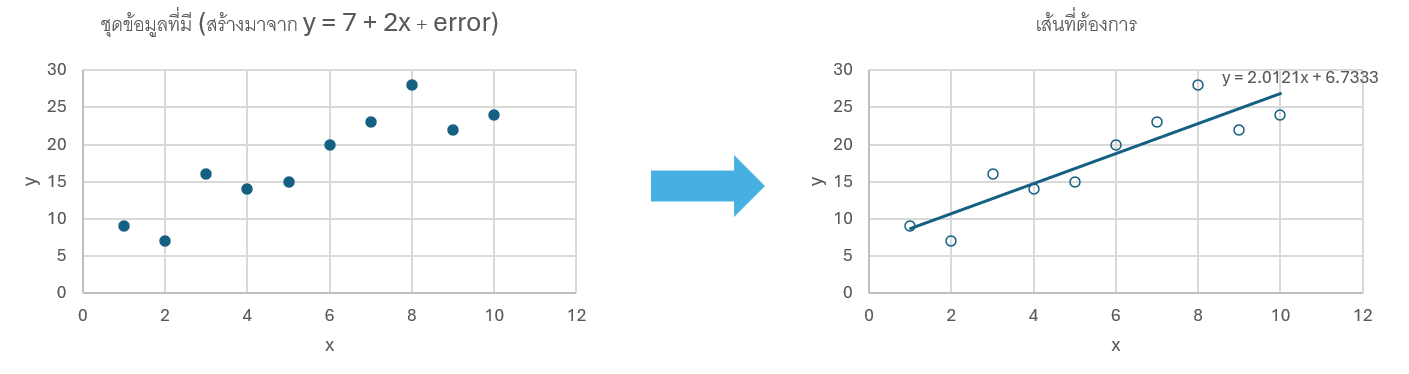
\includegraphics[width=1\linewidth]{regressionSample.png}
\end{figure}
\begin{tabular}{|c|c|}
    \hline
    $x$ & $y$ \\[0.05em] & \\ \hline
    1     & 9   \\[0.05em] & \\ \hline
    2     & 7    \\[0.05em] & \\ \hline
    3     & 16    \\[0.05em] & \\ \hline
    4     & 14   \\[0.05em] & \\ \hline
    5     & 15   \\[0.05em] & \\ \hline
    6     & 20   \\[0.05em] & \\ \hline
    7     & 23  \\[0.05em] &  \\ \hline
    8     & 28  \\[0.05em] &  \\ \hline
    9     & 22   \\[0.05em] & \\ \hline
    10    & 24   \\[0.05em] & \\ \hline
\end{tabular}\\

\section{การประเมิณผลความแม่นยำในการทำนาย}
อย่างที่ได้กล่าวไปก่อนหน้านี้ว่าเราไม่สามารถระบุได้ว่าตัวแบบใดเป็นตัวแบบที่ดีที่สุด เพราะตัวแบบในการทำนายที่ดีขึ้นอยู่กับข้อมูลที่มีว่ามีลักษณะข้อมูลเป็นอย่างไร ตัวแบบเดียวกันอาจจะทำงานได้ดีในชุดข้อมูลหนึ่ง แต่อาจจะทำได้ไม่ดีในอีกชุดข้อมูลหนึ่ง เพราะฉะนั้น ในกระบวนการทำงานจริง จึงต้องมีการวัดผลเพื่อประเมิณความแม่นยำของตัวแบบเพื่อที่จะเปรียบเทียบความสามารถในการทำนายของแต่ละตัวแบบได้ ซึ่งแนวคิดหลักของการวัดผลคือการใช้ค่า\textbf{ความคลาดเคลื่อน} (error) เพื่อเป็นตัวบอกว่าสิ่งที่ตัวแบบทำนายออกมาได้คลาดเคลื่อนออกไปจากค่าจริงเท่าใด
\[
\text{ค่าความคลาดเคลื่อนดิบ} = \left|\text{ค่าที่ตัวแบบทำนายได้} - \text{ค่าจริงจากชุดข้อมูล}\right|
\]
\begin{center}
	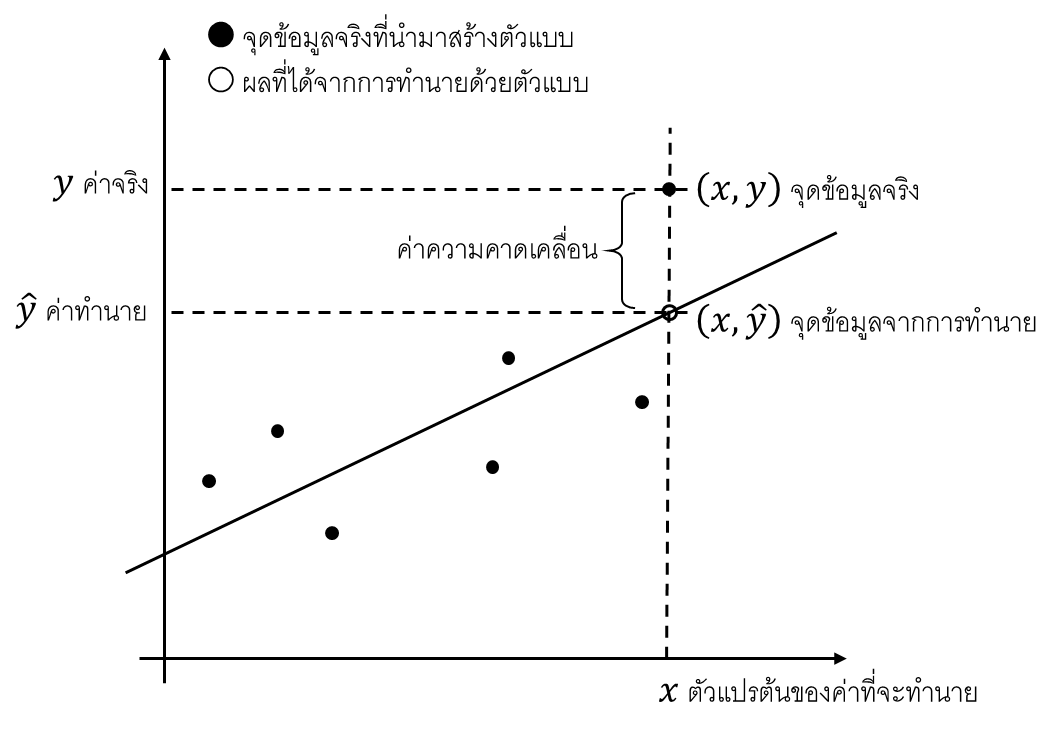
\includegraphics[width=0.5\linewidth]{image/error_in_forecasting}
\end{center}
ในหนังสือเล่มนี้ จะแบ่งการวัดผลออกเป็น 2 รูปแบบหลักได้แก่
\begin{enumerate}
	\item \textbf{การวัดผลด้วยมาตรวัดของข้อมูล}: เป็นการวัดผลที่มีหน่วยออกมาเป็นหน่วยเดียวกันกับข้อมูลที่เราต้องการจะทำนาย โดยต้องการวัดระยะห่าง มีข้อดีในแง่การแสกงค่าคาดเคลื่อนจริง ๆ เช่นทำนายคลาดเคลื่อนไปกี่บาท มักถูกใช้ในการเปรียบเทียบระหว่างตัวแบบต่าง ๆ บนข้อมูลชุดเดียวกัน โดยจะกล่าวถึง
	\begin{itemize}
		\item ค่าเฉลี่ยของความผิดพลาดสัมบูรณ์ (mean absolute error: MAE)
		\item ค่ารากที่สองของค่าเฉลี่ยของความผิดพลาดกำลังสอง (root mean squared error: RMSE)
	\end{itemize}
	\item \textbf{การวัดผลเชิงสัมพัทธ์}: เป็นการวัดผลในเชิงการหาร้อยละเทียบเคียงกับค่าจริงว่าคลาดเคลื่อนไปกี่เปอร์เซนต์ ซึ่งวิธีการนี้มักใช้กับชุดข้อมูลที่ความรุนแรงของการคลาดเคลื่อนขึ้นอยู่กับขนาดของค่าจริง กล่าวคือการคาดเคลื่อนด้วยปริมาณหนึ่งตอนที่ค่าจริงมีค่าน้อย ๆ จะรุนแรงกว่าการคาดเคลื่อนขนาดเดียวกันเมื่อค่าจริงมีค่ามาก ๆ (ตัวอย่างเช่น เงินหาย 9 บาทจาก 10 บาท กับเงินหายไป 9 บาทจาก 1 ล้านบาท) อีกทั้งยังเป็นค่าความคลาดเคลื่อนที่ใช้เพื่อการเปรียบเที่ยบการทำงานของตัวแบบในต่างชุดข้อมูลที่อาจจะมีค่าที่ต้องการทำนายอยู่ในคนละมาตรวัดกัน โดยจะกล่าวถึง
	\begin{itemize}
		\item ค่าเฉลี่ยของความผิดพลาดสัมพัทธ์ (mean absolute percentage error: MAPE)
		\item ค่าเฉลี่ยของความผิดพลาดสัมบูรณ์ที่ปรับมาตราส่วน (mean absolute scaled error: MASE)
	\end{itemize}
\end{enumerate}

\begin{definition}
	{mean absolute error}{}
	\[
	MAE = \frac{1}{n}\sum_{i=1}^{n}{|\hat{y}_i - y_i|}
	\]
\end{definition}

\begin{definition}
	{root mean squared error}{}
	\[
	RMSE = \sqrt{\frac{1}{n}\sum_{i=1}^{n}{(\hat{y}_i - y_i)^2}}
	\]
	และในบางครั้ง อาจมีการใช้ MSE ซึ่งคือ
	\[
	MSE = \frac{1}{n}\sum_{i=1}^{n}{(\hat{y}_i - y_i)^2}
	\]
	แต่สิ่งที่ต้องระวังตอนอ่านค่าคือค่าที่ได้จะอยู่ในหน่วยกำลังสองของหน่วยเดิม (เช่นหน่วย $\text{บาท}^2$) ซึ่งไม่ได้มีความหมายในโลกจริง
\end{definition}

\begin{definition}
	{mean absolute percentage error}{}
	\[
	MAPE = \frac{1}{n}\sum_{i=1}^{n}{\left|  \frac{\hat{y}_i - y_i}{y_i} \right|\times 100\% }
	\]
\end{definition}

\begin{definition}
	{mean absolute scaled error}{}
	สำหรับการทำการถดถอยเชิงเส้นเมื่อเทียบกับการทำนายด้วยการหยิบแต่ค่าเฉลี่ยมาเป็นค่าทำนาย
	\[
	MASE = {\frac{\sum_{i=1}^{n}|\hat{y}_i - y_i|}{\sum_{i=1}^{n}|\bar{y}-y_i|}  }
	\]
	
	สำหรับอนุกรมเวลาเมื่อเทียบกับการทำนายด้วยการหยิบค่าของครั้งก่อนหน้ามาเป็นค่าทำนายของครั้งปัจจุบัน
	\[
	MASE = {\frac{\frac{1}{n}\sum_{i=1}^{n}|\hat{y}_i - y_i|}{\frac{1}{T-1}\sum_{t=2}^{T}|y_t - y_{t-1}|}  }
	\]
	สำหรับการวัดผลด้วย MASE นั้น เราสามารถปรับเปลี่ยนวิธีการประมาณค่าตัวเทียบ (ตัวส่วน) เป็นตัวแบบแบบอื่นได้เช่นกัน เพียงแต่ 2 สูตรด้านบนเป็นการเทียบจากตัวแบบที่ง่ายที่สุดที่มักจะนึกถึงกันเป็นอันดับแรกตอนทำนาย
\end{definition}
\newpage
\begin{example}
	{การวัดผลอนุกรมเวลา}{}
	จากตารางการทำตัวแบบอนุกรมเวลาแบบต่าง ๆ ที่ทำมาในตัวอย่างที่ผ่าน ๆ มา จงวัดผลค่าความคลาดเคลื่อน MAE, RMSE, MAPE, MASE ของแต่ละตัวแบบ โดยสมมติเพิ่มว่าค่าจริงของเดือนที่ 7 มีค่าเท่ากับ 1200 (และเพื่อความสะดวกในการคำนวณ จึงขอปัดค่าทำนายให้เป็นจำนวนเต็ม)
\end{example}

วิธีค่าเฉลี่ย\\
\begin{tabular}{|c|c|c|}
	\hline
	เดือน & ยอดขายจริง & ค่าทำนาย \\ \hline
	1     & 800        & -              \\ \hline
	2     & 900        & 800           \\ \hline
	3     & 800        & 850           \\ \hline
	4     & 1000       & 833           \\ \hline
	5     & 1000       & 875           \\ \hline
	6     & 1300       & 900           \\ \hline
	7     & 1200       & 967           \\ \hline
\end{tabular}
\vspace{1cm}\\
วิธีเฉลี่ยเคลื่อนที่ 3 เดือน\\
\begin{tabular}{|c|c|c|}
	\hline
	เดือน & ยอดขายจริง & ค่าทำนาย \\ \hline
	1     & 800        &   -            \\ \hline
	2     & 900        &  -          \\ \hline
	3     & 800        &   -         \\ \hline
	4     & 1000       & 833           \\ \hline
	5     & 1000       & 900           \\ \hline
	6     & 1300       & 933           \\ \hline
	7     & 1200       & 1100           \\ \hline
\end{tabular}
\vspace{1cm}\\
วิธีเฉลี่ยเคลื่อนที่ 4 เดือน\\
\begin{tabular}{|c|c|c|}
	\hline
	เดือน & ยอดขายจริง & ค่าทำนาย \\ \hline
	1     & 800        &  -             \\ \hline
	2     & 900        &  -          \\ \hline
	3     & 800        &   -         \\ \hline
	4     & 1000       &  -          \\ \hline
	5     & 1000       & 875           \\ \hline
	6     & 1300       & 925           \\ \hline
	7     & 1200       & 1025           \\ \hline
\end{tabular}
\vspace{1cm}\\
วิธีค่าเฉลี่ยถ่วงน้ำหนัก 3 เดือน\\
\begin{tabular}{|c|c|c|}
	\hline
	เดือน & ยอดขายจริง & ค่าทำนาย \\ \hline
	1     & 800        &  -             \\ \hline
	2     & 900        &  -          \\ \hline
	3     & 800        &  -          \\ \hline
	4     & 1000       & 833           \\ \hline
	5     & 1000       & 917           \\ \hline
	6     & 1300       & 967           \\ \hline
	7     & 1200       & 1150           \\ \hline
\end{tabular}
\vspace{1cm}\\
วิธีค่าเฉลี่ยถ่วงน้ำหนัก 4 เดือน\\
\begin{tabular}{|c|c|c|}
	\hline
	เดือน & ยอดขายจริง & ค่าทำนาย \\ \hline
	1     & 800        &   -            \\ \hline
	2     & 900        &   -         \\ \hline
	3     & 800        &  -          \\ \hline
	4     & 1000       &  -          \\ \hline
	5     & 1000       & 900           \\ \hline
	6     & 1300       & 950           \\ \hline
	7     & 1200       & 1100           \\ \hline
\end{tabular}
\vspace{1cm}\\
วิธีปรับเรียบแบบเอ็กโพเนนเชียล โดย $\alpha=0.3$\\
\begin{tabular}{|c|c|c|}
	\hline
	เดือน & ยอดขายจริง & ค่าทำนาย \\ \hline
	1     & 800        & 800              \\ \hline
	2     & 900        & 800           \\ \hline
	3     & 800        & 830           \\ \hline
	4     & 1000       & 821           \\ \hline
	5     & 1000       & 875           \\ \hline
	6     & 1300       & 912           \\ \hline
	7     & 1200       & 1029           \\ \hline
\end{tabular}
\vspace{5cm}\\
วิธีปรับเรียบแบบเอ็กโพเนนเชียล โดย $\alpha=0.8$\\
\begin{tabular}{|c|c|c|}
	\hline
	เดือน & ยอดขายจริง & ค่าทำนาย \\ \hline
	1     & 800        & 800              \\ \hline
	2     & 900        & 800           \\ \hline
	3     & 800        & 880           \\ \hline
	4     & 1000       & 806           \\ \hline
	5     & 1000       & 964           \\ \hline
	6     & 1300       & 975           \\ \hline
	7     & 1200       & 1222           \\ \hline
\end{tabular}
\newpage
\begin{example}
	{การวัดผลการถดถอยเชิงเส้น}{}
	จากตัวอย่างการหาตัวแบบการถดถอยเชิงเส้นในตัวอย่าง \ref{ex:regression1} จงวัดผลความคลาดเคลื่อน MAE, RMSE, MAPE, MASE (ในทำนองเดียวกัน ถ้าเป็นการคำนวณมือให้ปัดเป็นจำนวนเต็มเพื่อคิดเลขได้ จะได้คำนวณได้สะดวก)
\end{example}
\begin{tabular}{|c|c|c|}
	\hline
	$x$ & $y$ & $\hat{y}$\\[0.05em] & &.........\\ \hline
	1     & 9   & \\[0.05em] & &\\ \hline
	2     & 7    & \\[0.05em] & &\\ \hline
	3     & 16    & \\[0.05em] & &\\ \hline
	4     & 14   & \\[0.05em] & &\\ \hline
	5     & 15   & \\[0.05em] & &\\ \hline
	6     & 20   & \\[0.05em] & &\\ \hline
	7     & 23  & \\[0.05em] &  &\\ \hline
	8     & 28  & \\[0.05em] &  &\\ \hline
	9     & 22   & \\[0.05em] & &\\ \hline
	10    & 24  &  \\[0.05em] & &\\ \hline
\end{tabular}

\newpage
\section{การใช้ Excel เพื่อช่วยคำนวณหาตัวแบบต่าง ๆ}
\newpage